\documentclass[12pt,preprint]{aastex}

\include{vc}

\usepackage{color,hyperref}
\definecolor{linkcolor}{rgb}{0,0,0.5}
\hypersetup{colorlinks=true,linkcolor=linkcolor,citecolor=linkcolor,
            filecolor=linkcolor,urlcolor=linkcolor}
\usepackage{url}
\usepackage{amssymb,amsmath}
\usepackage{subfigure}

\usepackage{listings}
\definecolor{lbcolor}{rgb}{0.9,0.9,0.9}
\lstset{language=Python,
        basicstyle=\footnotesize\ttfamily,
        belowskip=-3pt,
        showspaces=false,
        showstringspaces=false,
        tabsize=2,
        breaklines=false,
        breakatwhitespace=true,
        identifierstyle=\ttfamily,
        keywordstyle=\bfseries\color[rgb]{0.133,0.545,0.133},
        commentstyle=\color[rgb]{0.133,0.545,0.133},
        stringstyle=\color[rgb]{0.627,0.126,0.941},
    }

\usepackage{algorithmic,algorithm}
\renewcommand{\algorithmicrequire}{\textbf{Input:}}
\renewcommand{\algorithmicensure}{\textbf{Output:}}

\newcommand{\project}[1]{{\sffamily #1}}
\newcommand{\ipython}{\project{IPython}}
\newcommand{\paper}{\textsl{Worksheet}}

\newcommand{\foreign}[1]{\emph{#1}}
\newcommand{\etal}{\foreign{et\,al.}}
\newcommand{\etc}{\foreign{etc.}}

\newcommand{\Fig}[1]{Figure~\ref{fig:#1}}
\newcommand{\fig}[1]{\Fig{#1}}
\newcommand{\figlabel}[1]{\label{fig:#1}}
\newcommand{\Tab}[1]{Table~\ref{tab:#1}}
\newcommand{\tab}[1]{\Tab{#1}}
\newcommand{\tablabel}[1]{\label{tab:#1}}
\newcommand{\Eq}[1]{Equation~(\ref{eq:#1})}
\newcommand{\eq}[1]{\Eq{#1}}
\newcommand{\eqalt}[1]{Equation~\ref{eq:#1}}
\newcommand{\eqlabel}[1]{\label{eq:#1}}
\newcommand{\Sect}[1]{Section~\ref{sect:#1}}
\newcommand{\sect}[1]{\Sect{#1}}
\newcommand{\App}[1]{Appendix~\ref{sect:#1}}
\newcommand{\app}[1]{\App{#1}}
\newcommand{\sectlabel}[1]{\label{sect:#1}}

\newcommand{\dd}{\ensuremath{\,\mathrm{d}}}
\newcommand{\bvec}[1]{\ensuremath{\boldsymbol{#1}}}

\begin{document}

\title{%
    Gaussian processes lab worksheet
}

\author{%
    Daniel~Foreman-Mackey\altaffilmark{1}
}
\altaffiltext{1}{Center for Cosmology and Particle Physics,
                 Department of Physics, New York University,
                 4 Washington Place, New York, NY, 10003, USA;
                 \url{danfm@nyu.edu}}

In this lab, we'll work through two example problems in Gaussian process
regression using Python.
In the first example, we'll get our feet wet by fitting a linear model to data
with correlated uncertainties and a small number of data points where
performance isn't a huge limiting factor.
Then, after benchmarking and optimizing the code, we'll fit for the location,
width and amplitude of a Gaussian ``feature'' imposed on a
not-entirely-trivial continuum function.
This example is similar to what you might want to do when fitting a spectral
feature or a simplified version of fitting the location and parameters of a
transiting exoplanet.

The lab is designed to be open-ended and the last sections should be
instructive even for students who are already familiar with the implementation
of Gaussian processes.
I've chosen to use Python for the lab because it is my programming language of
choice and because it is becoming commonly used in astronomy.
If you don't have experience coding in Python I've tried to include a lot of
skeleton code so you should still be able to make progress without getting too
caught up in that funny Python syntax.

\section{Fitting a line to data with correlated noise}

\subsection{Getting started}

For the first half of this section, we'll be working interactively so we'll
use the Hammer%
\footnote{\url{https://rcc.its.psu.edu/user_guides/systems/hammer/}} system
and the provided Python 2.7.3.
To get there, SSH using the command:
\begin{lstlisting}
% ssh -X YOUR_USER_NAME@hammer.rcc.psu.edu
\end{lstlisting}
At the prompt, enter your password and then load the modules that we'll need:
\begin{lstlisting}
% module load git
% module load python/2.7.3
\end{lstlisting}

The data and some skeleton code for this lab is available on GitHub%
\footnote{\url{https://github.com/dfm/gp}} and you can get it by running:
\begin{lstlisting}
% cd work
% git clone https://github.com/dfm/gp
% cd gp
\end{lstlisting}

If everything worked as planned, you should now be able to run Python (we'll
use \ipython\footnote{\url{http://ipython.org/}} for our interactive work) and
import the helper module:
\begin{lstlisting}
% ipython
>>> import gp
\end{lstlisting}
This module provides a few bells and whistles to help the lab run smoothly but
if you're interested, you should definitely check out the source code online
at \url{https://github.com/dfm/gp}.

\subsection{Working with the data}

You should now be able to load and plot the data:
\begin{lstlisting}
>>> x, y, yerr = gp.line.load_data()
>>> gp.line.plot_data(x, y, yerr)
\end{lstlisting}
The plot is generated using \project{matplotlib} and it should appear in a
window on your machine looking something like \fig{line-data}.

\begin{figure}[htbp]
\begin{center}
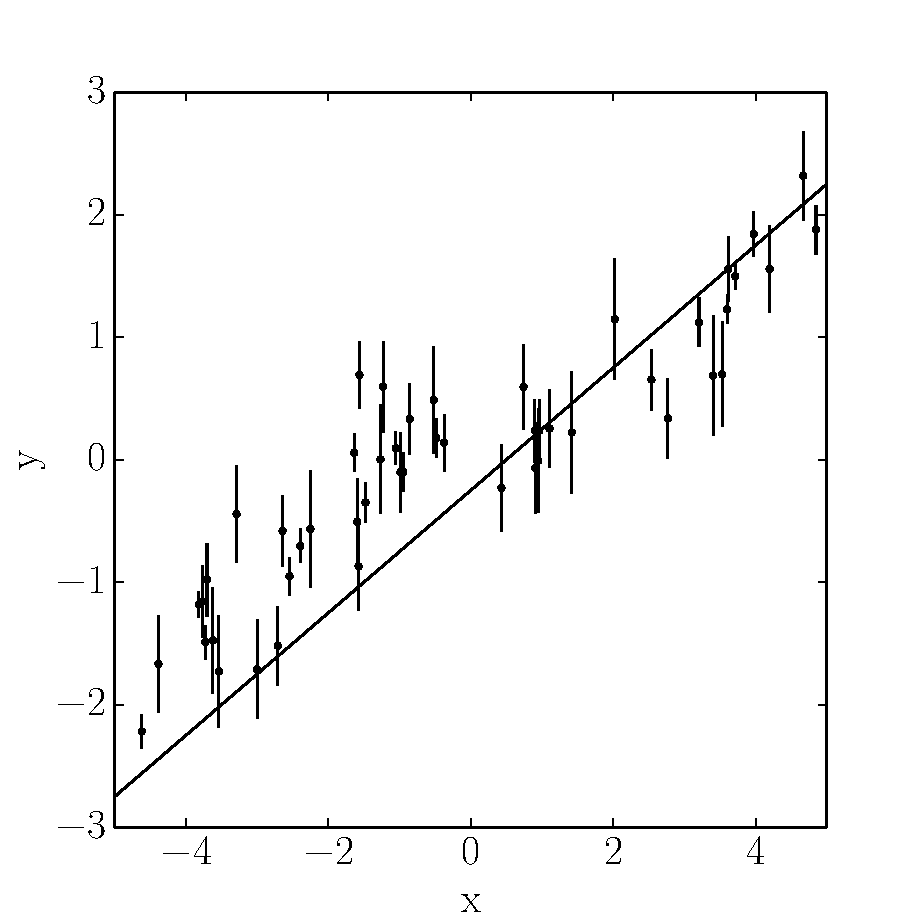
\includegraphics[width=0.5\textwidth]{figures/line_data.pdf}
\end{center}
\caption{%
The points with error bars are the data for the linear fit section and the
black line shows the true model that was used to generate the data.
\figlabel{line-data}}
\end{figure}

\subsection{Linear least squares}

Now we'll run our baseline model: linear least squares.
In this model, we'll assume that the uncertainties are known, independent, and
Gaussian.
For simplicity, I've implemented this model for you even though it's only a
couple of lines of code%
\footnote{\url{https://github.com/dfm/gp/blob/master/gp/line/lls.py}}.
You can run it as follows:
\begin{lstlisting}
>>> mu, cov = gp.line.least_squares(x, y, yerr)
\end{lstlisting}
This function returns the mean and covariance of the Gaussian posterior
constraints on the slope $m$ and intercept $b$ of the line and if you print
these at the command line, you should see
\begin{lstlisting}
>>> print(mu)
[ 0.36482633  0.1229681 ]
>>> print(cov)
[[  1.10886015e-04   4.41514429e-05]
 [  4.41514429e-05   9.78666012e-04]]
\end{lstlisting}
which is very far away from the true values
\begin{eqnarray}
m = 0.5 &\mathrm{and}& b = -0.25 \quad.
\end{eqnarray}

To demonstrate just how bad this result is, let's plot it on top of the data.
To do this, we need to generate a list of samples (let's say 20,000, this
time) from this posterior distribution.
Luckily, \project{numpy} has a built in function for generating samples from a
multivariate Gaussian
\begin{lstlisting}
>>> import numpy as np
>>> samples = np.random.multivariate_normal(mu, cov, 20000)
\end{lstlisting}
And then we can plot the results:
\begin{lstlisting}
>>> gp.line.plot_results(x, y, yerr, samples)
\end{lstlisting}
This should show two figures.
The first should look something like \fig{line-lls-triangle}, showing the
constraints in the two-dimensional parameter space.
The true value is so far that it isn't even visible on this plot.
The second figure should look something like \fig{line-lls} where the
predicted line is shown as the red area.

This result is very precise but (since we know the true value) we can see that
it is also very inaccurate.

\begin{figure}[htbp]
\begin{center}
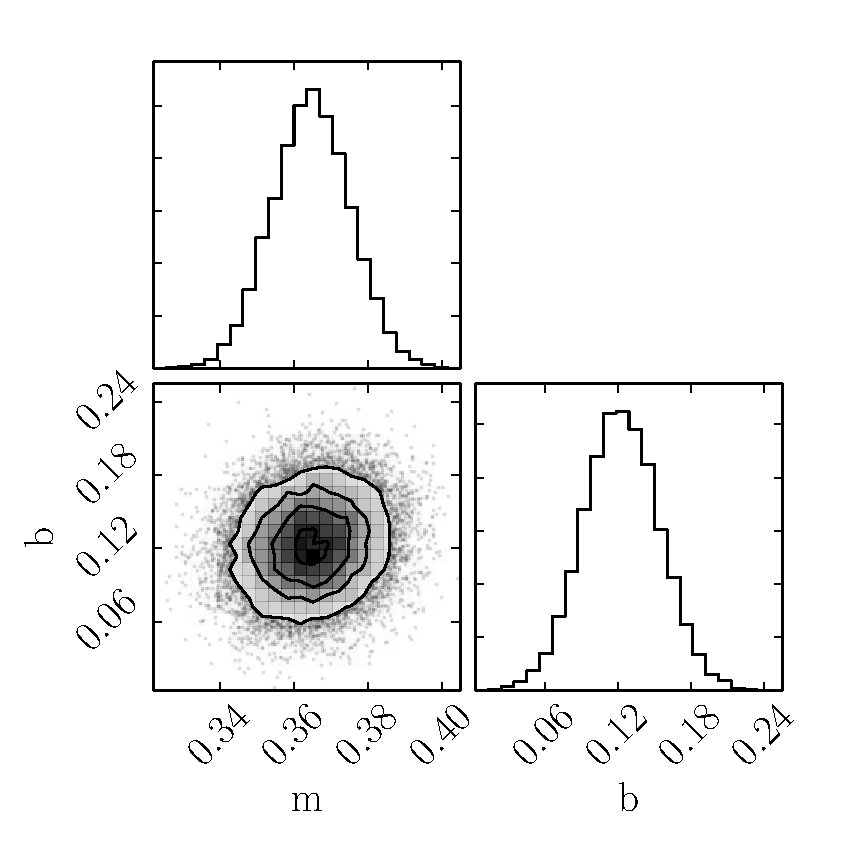
\includegraphics[width=0.5\textwidth]{figures/line_lls_triangle.pdf}
\end{center}
\caption{%
\figlabel{line-lls-triangle}}
\end{figure}

\begin{figure}[htbp]
\begin{center}
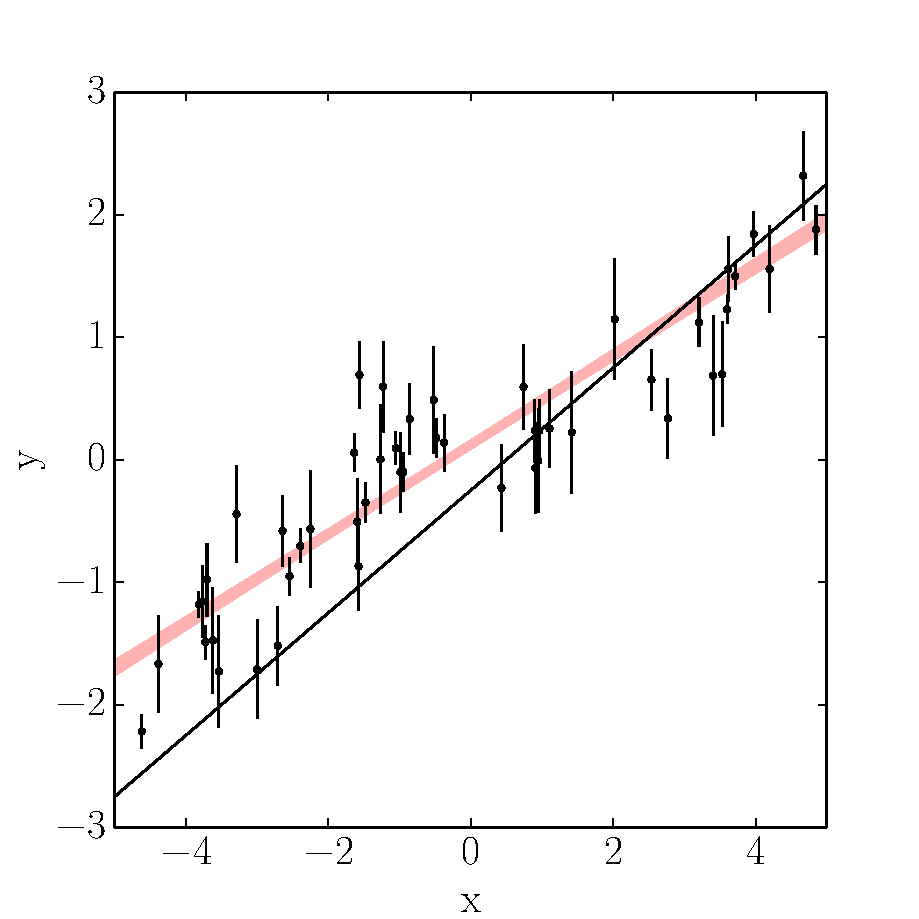
\includegraphics[width=0.5\textwidth]{figures/line_lls.pdf}
\end{center}
\caption{%
\figlabel{line-lls}}
\end{figure}

\subsection{The Gaussian likelihood function}

Now let's implement the code for a Gaussian process.
The main thing that you need to do in this section is write the
(ln-)likelihood function.
What you need to do is convert the following equation to Python (I'll give
some pointers in a moment)
\begin{eqnarray}\eqlabel{lnlike}
\ln L - C &=& -\frac{1}{2}\,\bvec{r}^\mathrm{T}\,\bvec{K}^{-1}\,\bvec{r}
              -\frac{1}{2}\,\ln \det \bvec{K}
\end{eqnarray}
where $C$ is an irrelevant constant, $\bvec{r}$ is the residual vector, and
$\bvec{K}$ is the covariance matrix.
What we want is a function like
\begin{lstlisting}
def lnlike(r, K):
    ...
\end{lstlisting}
that takes in a vector \texttt{r} and a matrix \texttt{K} and returns the
right-hand side of \eq{lnlike}.
One thing to think about while you do this is that you should \emph{never}
invert a matrix.
Instead, to find $\bvec{x}$ in this equation
\begin{eqnarray}
\bvec{x} = \bvec{K}^{-1}\,\bvec{r} &\to& \bvec{r} = \bvec{K}\,\bvec{x}
\end{eqnarray}
you should use something like the \project{numpy} function
\texttt{np.linalg.solve}\footnote{\url{%
http://docs.scipy.org/doc/numpy/reference/generated/numpy.linalg.solve.html}}.
Another useful function is \texttt{np.linalg.slogdet}\footnote{\url{%
http://docs.scipy.org/doc/numpy/reference/generated/numpy.linalg.slogdet.html%
}}.
that computes the sign and ln-determinant of a matrix.
This is much more numerically stable than computing the determinant directly
and in \eq{lnlike} we only ever use the ln-determinant.

Your code should roughly follow the format of the pseudo-code given below in
Algorithm~\ref{algo:lnlike}:
\begin{algorithm}
\caption{Pseudo-code for computing the Gaussian process likelihood.
         \label{algo:lnlike}}
\begin{algorithmic}[1]

\REQUIRE Residual vector \bvec{r}; covariance matrix \bvec{K}
\ENSURE The ln-likelihood (up to a constant)
\STATE $\bvec{\alpha} \gets \mathtt{np.linalg.solve}(\bvec{K},\,\bvec{r})$
\STATE $(s,\,d) \gets \mathtt{np.linalg.slogdet}(\bvec{K})$
\RETURN $-0.5\,\left(\bvec{r}\cdot\bvec{\alpha} + d\right)$

\end{algorithmic}
\end{algorithm}

To check that the likelihood function that you wrote is correct, save it in a
Python file (called something like \texttt{gp\_likelihood.py}, for example)
with the following format:
\begin{lstlisting}[frame=single]
# The file gp_likelihood.py

import gp
import numpy as np

def lnlike(r, K):
    # Write the code for Algorithm 1 here

gp.utils.test_lnlike(lnlike)
\end{lstlisting}
Then, when you run this script
\begin{lstlisting}
% python gp_likelihood.py
\end{lstlisting}
it will raise an error if there is a problem with your code.

Next, we need to implement the kernel function.
This will take in a distance $\Delta x$ and a vector of parameters
$(\alpha, \tau)$, and return
\begin{eqnarray}\eqlabel{kernel}
k(\Delta x) &=& \alpha^2\,\exp \left(-\frac{\Delta x^2}{2\,\tau^2}\right) \quad.
\end{eqnarray}
To do this, add the following skeleton code to the bottom of of your source
code file:
\begin{lstlisting}[frame=single]
# Continuation of the file gp_likelihood.py

def kernel(params, dx):
    # Implement the kernel equation here

gp.utils.test_kernel(kernel)
\end{lstlisting}
and implement \eq{kernel} as indicated.
\emph{Note: the} \texttt{kernel} \emph{function should be able to handle
\project{numpy} arrays so you should use the function} \texttt{np.exp}
\emph{for exponentiation.}
If you run your script again:
\begin{lstlisting}
% python gp_likelihood.py
\end{lstlisting}
it will fail if the kernel function isn't implemented correctly.

\subsection{Benchmarking}

Let's take a moment now to benchmark our code.







All of the code used in the making of this worksheet is available from
\url{https://github.com/dfm/gp} under the MIT open-source software license.
This version was generated with git commit \texttt{\githash} (\gitdate).

\newcommand{\arxiv}[1]{\href{http://arxiv.org/abs/#1}{arXiv:#1}}
\begin{thebibliography}{}\raggedright

\bibitem[Ambikasaran \etal(2014)]{dfm-gp}
Ambikasaran, S., Foreman-Mackey, D., Greengard, L., Hogg, D.~W.,
\& O'Neil, M.\ 2014, \arxiv{1403.6015}

\bibitem[Rasmussen \& Williams(2006)]{gp}
Rasmussen, C.~E. \& Williams, C.~K.~I.\ 2006
Gaussian Processes for Machine Learning, MIT Press
(\href{http://www.gaussianprocess.org/gpml/}{online})

\end{thebibliography}

\end{document}
